\documentclass[a4paper,12pt]{article}

%------------------------------------------------------------------------------------------%
% Déclaration des packages
%------------------------------------------------------------------------------------------%

\usepackage[french]{babel}
\frenchbsetup{StandardLists=true}
\usepackage{enumitem}
\usepackage[T1]{fontenc}
\usepackage{geometry} % pour gérer les dimensions des marges
\usepackage{eso-pic} % pour dessiner la marge
\usepackage{lipsum} % pour générer du contenu texte
\usepackage[cyr]{aeguill} % Police vectorielle TrueType, guillemets fran¸cais
\usepackage{epsfig} % pour g´erer les images
\usepackage{amsmath, amsthm} % tr`es bon mode math´ematique
\usepackage{amsfonts,amssymb}% permet la definition des ensembles
\usepackage{float} % pour le placement des figure
\usepackage{url} 
\usepackage[utf8]{inputenc}
\usepackage{amssymb}
\usepackage{graphicx}
\usepackage{ulem}
\usepackage{array}	
\usepackage{listings}
\usepackage{siunitx}
\usepackage{fancybox}
\usepackage{wrapfig}
\usepackage{caption}
 \usepackage{hyperref}
\usepackage{listings}
\usepackage{xcolor}


\title{Football predictor}
\geometry{top=25mm, bottom=25mm, left=20mm, right=1cm}
\setlength\headheight{10mm}
\DeclareUnicodeCharacter{2212}{-}
\renewcommand{\thefootnote}{\fnsymbol{footnote}}
\renewcommand{\thefootnote}{\fnsymbol{footnote}}
\newcommand{\chatgptprompt}[1]{
    \vspace{10pt}
    \noindent\textbf{ChatGPT Prompt:}\\
    \fbox{
        \parbox{\textwidth}{
            \texttt{#1}
        }
    }
    \vspace{10pt}
}



\geometry{a4paper, margin=1in}

\title{\huge\bf Football Predictor}
\date{19/11/2023}
\author{CouscousSamba} 
\begin{document}

\begin{titlepage}
    \begin{center}
        
\includegraphics[width=0.3\textwidth]{images/DS4HlogocouleurFR.png} \hfill
        
\includegraphics[width=0.3\textwidth]{images/logo_master.png} \hfill
        
\includegraphics[width=0.23\textwidth]{images/tampon-3IA.png}
        
        \vspace{1.5cm}
        
        \textbf{\LARGE Université C\^ote d'Azur}
        
        \vspace{0.5cm}
        
        \textbf{\Large Master Informatique, parcours Intelligence Artificielle}
        
        \vspace{1.5cm}
        
        \textbf{\Large Project report}
        
        \vspace{0.5cm}
        
        \rule{\linewidth}{0.5mm} \\[0.4cm]
        {\LARGE \bfseries Football Predictor \\[0.2cm]}
        \rule{\linewidth}{0.5mm} \\[1.5cm]
        
        \textbf{Authors:} \\
        BOULLI Marouan, BAPTISTA Rafael and HADDOU Amine   \\
        
        \vspace{0.8cm}
        
        \textbf{Supervised by:} \\
        FORMENTI Enrico\\
        
        \vspace{1.5cm}
        
        \textbf{Due Date:} \\
        \today
        
    \end{center}
\end{titlepage}
\newpage
\maketitle
\tableofcontents

\newpage
\section{Project}

The "Football Predictor" project is undertaken as part of the Neural Network course, under the guidance of Professor Formenti Enrico. The primary objective is to develop an artificial intelligence model capable of predicting the outcomes of football matches, specifically identifying the winning team. This endeavor leverages two datasets, which will be detailed in the subsequent sections, to train and optimize the predictive model.

\section{Project Presentation}

This project aims to utilize machine learning techniques to predict football match outcomes, blending the realms of sports analytic and artificial intelligence. The foundation for our predictions is based upon two datasets - the "International football results from 1872 to 2023" and the "FIFA World Ranking 1992-2023." The former comprises over 45,000 international football match results, spanning from the inaugural match in 1872 to 2023, sourced from various international football associations. The latter dataset contains FIFA rankings for men's national teams from 1992 to (July) 2023. These datasets, referred to as "results" and "ranking," respectively, serve as the building blocks for our predictive model.\\

In the end, we should be able to predict match results and the winner of a championship.\\

To that end, we followed 3 steps:
\begin{enumerate}
    \item \textbf{Data preprocessing}.
    \item \textbf{Models training and evaluation}.
    \item \textbf{User interface development}.
\end{enumerate}

The source code is available at the following github repository: \href{https://github.com/H4znow/Football_match_results_predictor}{Football match result predictor}

\subsection{Members}

The collaborative effort behind the Football Predictor project is led by the following team members:
\begin{itemize}
    \item Marouan Boulli
    \item Rafael Baptista
    \item Amine Haddou
\end{itemize}
Each member brings a unique set of skills and expertise to the project, fostering a diverse and capable team.

\subsection{Datasets} 

The project relies on two key datasets obtained from Kaggle's website:
\begin{enumerate}
    \item "International football results from 1872 to 2023," available for download \href{https://www.kaggle.com/datasets/martj42/international-football-results-from-1872-to-2017}{here}.
    \item "FIFA World Ranking 1992-2023," accessible \href{https://www.kaggle.com/datasets/cashncarry/fifaworldranking}{here}.
\end{enumerate}
The first dataset encompasses a comprehensive collection of over 45,000 international football match results, spanning from the inception of official matches in 1872 to 2023, sourced from diverse international football associations. The second dataset provides FIFA rankings for men's national teams from 1992 to (July) 2023. These datasets, denoted as "results" and "ranking," form the cornerstone for our predictive modeling efforts.

\section{Organisation}

\subsection{GitHub} 

To ensure efficient collaboration and version control, we employ GitHub as a central repository for our project. While most work is conducted locally using notebooks (due to Git merge challenges with notebooks), regular updates are pushed by a designated team member to maintain the GitHub repository's currency.

\subsection{Kanban Board} 

Project management is facilitated through a Kanban board, which serves as the organizational backbone for our team. Tasks are assigned to each team member, providing a comprehensive overview of the project's progress and enabling individuals to clearly understand their responsibilities.

\subsection{Discord} 

Discord acts as the primary communication tool for our team. We have established a dedicated server where regular video conferences are held, fostering real-time communication and collaboration. The platform is also utilized for sharing ideas and progress updates, providing a space for constructive debates on various algorithms and methodologies.

\section{Preprocessing}

In this section, we delve into the preprocessing steps applied to the datasets.

\subsection{Fixing Country Names}

The dataset posed some challenges with inconsistent country names, including countries that no longer exists, those that underwent name changes, and variations in syntax. To address this, we employed two methods:\\

1) Utilizing the following ChatGPT prompt among some others that are included in this one 
\newpage
\chatgptprompt{Instructions: \
You are an expert specializing in modern geography and country names, as well as football (soccer). Your task is to process a list of countries provided in various languages. Some of these countries may have specific conditions or requirements that need to be addressed. Here are the instructions to be followed: \
1. You will receive a list of countries in different languages.
2. Some of these countries may no longer exist, have different names, appear multiple times in different formats, be in a non-simplified form (e.g., IR Iran instead of Iran), or not have a national football team.
3. These countries will be referred to as "false countries."
4. Your output should be in JSON format, where each key represents a "false country," and its corresponding value indicates the correct actual name in English.
5. If a "false country" doesn't have a national football team, its value in the JSON should be "None." \
Please ensure that your response strictly adheres to the provided instructions and only includes the requested JSON output.}


we generated a dictionary to replace problematic country names with correct ones (e.g., URSS -> Russia, IR IRAN -> IRAN, Reunion -> France).\\

2) Mapping countries in the datasets using \textit{Pandas dataframe.replace()}, the new DataFrame contains the official names of all countries. This process homogenized the names using abbreviations, and we dropped countries for which we lacked information.

\subsection{Choosing a Year Cut-off}

After thorough consideration, we opted to establish a "cut-off year" based on the project's performance rather than alterations in country names. Data prior to the year 2000 is deemed largely irrelevant due to the following reasons:\\
\begin{itemize}
    \item Matches from that era have minimal impact on current game outcomes due to their age.
    \item Significant changes in game dynamics and player preparation over the years render comparisons between past and present matches less meaningful.
    \item The structure of competitions has undergone substantial transformations, making team performances from the past less indicative of their current capabilities.
\end{itemize}


This initial cut-off year allows us to filter out less relevant historical data. Subsequently, we plan to fine-tune the cut-off year further to enhance the precision of our predictive model.


\subsection{Features}

In the process of constructing our predictive model, not all features in the dataset prove to be relevant. As such, a careful selection of the most meaningful features becomes imperative. While there is no universally perfect solution for feature selection, our approach involves leveraging our soccer expertise as fans to make informed choices.\\

Traditionally, machine learning tasks often require expert input for feature selection. In our case, we consider ourselves soccer enthusiasts with sufficient knowledge to make informed decisions regarding feature relevance.\\

Here is list of features before the modifications at \ref{fig:features_b4_modifications}.

\begin{figure}
  \centering
  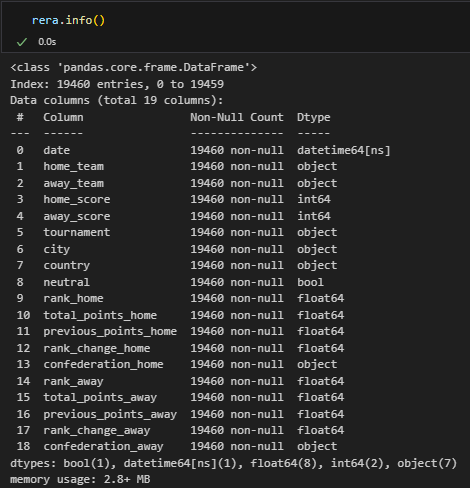
\includegraphics[height=9cm]{./images/features_b4_modifications.png}
  \caption{List of features before the modifications}
  \label{fig:features_b4_modifications}
\end{figure}

\subsubsection{New Features}

In our quest for optimal feature selection, we introduce new features to enhance the predictive capabilities of our model.\\

\textbf{Winner Feature:}
The `winner` feature is introduced as an integer column with three distinct values: \{0, 1, 2\}.
\begin{itemize}
    \item \textbf{0:} Indicates that the {\it home\_team} has emerged victorious.
    \item \textbf{1:} Indicates that the {\it away\_team} has secured a win.
    \item \textbf{2:} Represents a draw, signifying that both teams have achieved an equal outcome.\\
\end{itemize}

\textbf{Average Goal Feature:}
We incorporate two new features, {\it home\_goals\_avg} and {\it away\_goals\_avg}, representing the average number of goals scored by the home and away teams, respectively, in their last 7 matches. This choice is grounded in the notion that observing the goal-scoring patterns over the most recent seven matches provides valuable insights into a team's current performance.\\

\textbf{Average Win Feature:}
To further enrich our feature set, we introduce two additional features, {\it home\_win\_avg} and {\it away\_win\_avg}. These columns represent the average number of victories for the home and away teams in their last 7 matches. This metric offers a snapshot of a team's recent success rate, helping to capture its current form over a reasonably recent timeframe.

\textbf{Last Five Confrontations:}
Finally, we find it valuable to compute the number of victories for each team in their last five matches. This addition is motivated by the common observation in soccer, where a team may have a higher statistical standing than its opponent but still faces a likelihood of losing. Such occurrences can be attributed to intangible factors like pressure, intensity, and the overall context of the game.


\subsubsection{Deleted Features}

In our pursuit of a more streamlined and effective model, we have opted to eliminate certain features to mitigate the risk of overfitting and enhance the interpretability of our results.\\

To identify the features slated for removal, we employ a combination of intuitive assessment of seemingly irrelevant features and mathematical insights \ref{fig:stats}. One crucial metric guiding our decisions is the correlation coefficient. The computed correlations on our dataset are presented in the figure at \ref{fig:corr_hm}.\\

\begin{figure}
  \centering
  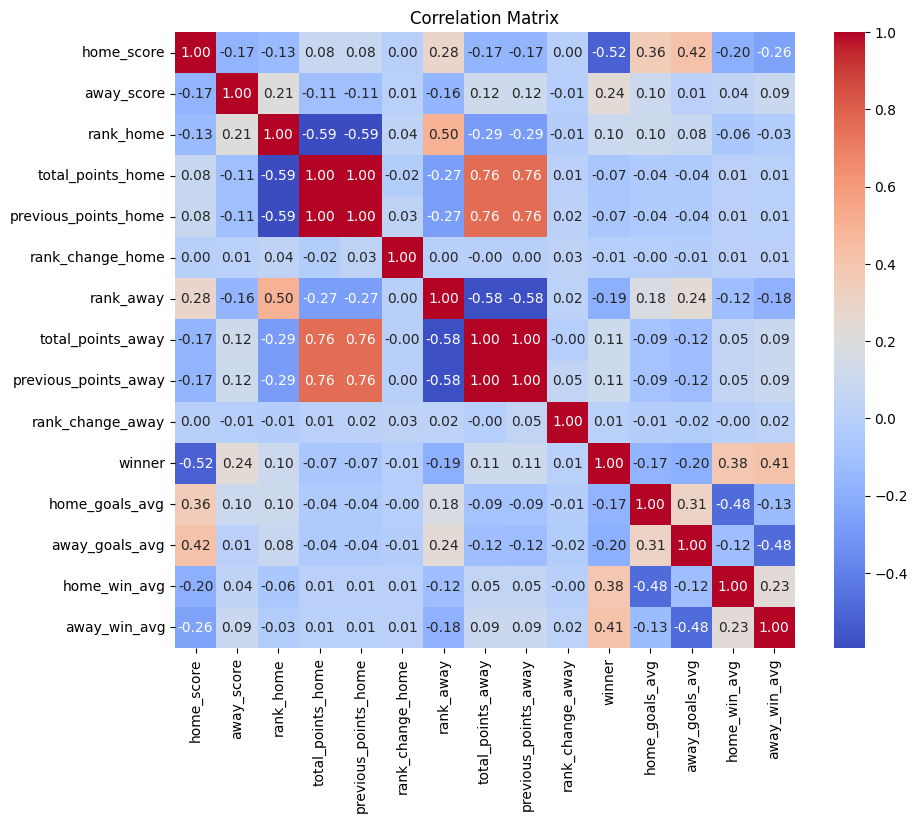
\includegraphics[width=0.8\textwidth]{./images/correlation_rera.png}  % Replace with the path to your image file
  \caption{The correlation heatmap of the dataset}
  \label{fig:corr_hm}
\end{figure}

\begin{figure}
  \centering
  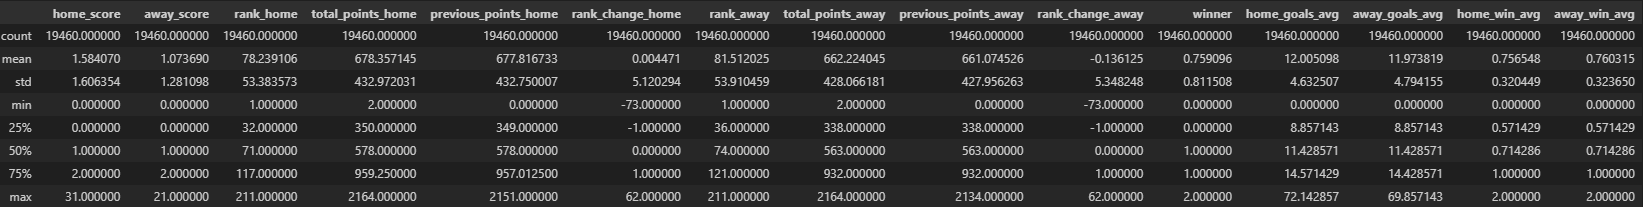
\includegraphics[width=0.8\textwidth]{./images/basic_stats_numerical_features.png}
  \caption{Basic statistics of numerical features}
  \label{fig:stats}
\end{figure}


{\bf City feature} : The feature is representing the location where a match is held, is deemed irrelevant to our analysis given the focus on national teams. Consequently, we have decided to drop this feature. The city where a match is played is considered inconsequential, as the outcome of national team matches is influenced more significantly by the country in which they are contested.\\

{\bf Country feature} : In a similar vein, we have chosen to discard the {\it country} column. The presence of a {\it neutral} column renders this redundant. If the match is not set as neutral (neutral = false), it is held in the home country. If it is, it is played in another country worldwide. The distinction between specific countries does not significantly impact the analysis in this context.\\

{\bf home\_score and away\_score features} : Furthermore, we will exclude the {\it home\_score} and {\it away\_score} features since we already have the {\it winner}, {\it home\_goals\_avg}, and {\it away\_goals\_avg} features. The introduction of average goal features provides a more nuanced perspective on team performance, considering that the number of goals alone may not fully capture a team's overall effectiveness. By removing the score columns, we aim to enhance the model's generalization capability and reduce the risk of overfitting. Anyway, the scores should not be present in the features since the column "winner" (label) has been created using the scores.\\

{\bf previous\_points\_home and previous\_points\_away Features} : As depicted in the correlation heat map \ref{fig:corr_hm}, \textit{previous\_points\_home} and \textit{previous\_points\_away} are respectively highly correlated with \textit{total\_points\_home} and \textit{total\_points\_away}. Over multiple matches, the number of points does not vary significantly, potentially explaining this correlation. We posit that the total number of points alone suffices, rendering the information from \textit{previous\_points} redundant, despite its slight variations.


\subsubsection{Standardization}

Standardization is a crucial preprocessing step in machine learning that aims to bring numerical features to a common scale, ensuring that they contribute equally to the model's training process.\\

In our context, standardizing the numerical data involves transforming each feature such that it has a mean of 0 and a standard deviation of 1. This not only removes potential biases introduced by different measurement units but also facilitates a more stable and efficient convergence during the training phase.\\

By standardizing the numerical features, we create a more uniform and fair representation of their influence on the model, promoting a robust and unbiased learning process.

\subsubsection{Encoding String and Boolean Type Features}

In our effort to optimize the model's performance, we considered encoding country names to address the challenges posed by String-type data. For instance, Germany might be represented as 0, England as 1, and France as 2.\\

Two primary encoding methods, Hotcoding and encoding, were evaluated. While the former initially seemed more logical, it resulted in an unwieldy number of new columns, unnecessarily complicating the model.\\

As a result, we decided on encoding. The columns selected for encoding include: \textit{home\_team}, \textit{away\_team}, \textit{confederation\_home}, \textit{confederation\_away}, and \textit{neutral}.\\

However, subsequent research revealed that for Principal Component Analysis (PCA) to be efficient, it is advisable to drop all categorical features, as PCA relies on the variation of numerical data. Consequently, encoding is unnecessary in our particular case.


\subsubsection{Dimensionality Reduction}

Dimensionality reduction is a technique used to decrease the number of features in a dataset while retaining crucial information. This approach serves various purposes, including reducing model complexity, enhancing the performance of learning algorithms, and facilitating data visualization.\\

To implement dimensionality reduction, we will employ the Principal Component Analysis (PCA) algorithm. Specifically, we are applying PCA to our encoded dataframe, \texttt{rera\_standardized\_encoded}, to determine the optimal value for the hyperparameter \texttt{n\_component}. This identified value will subsequently be incorporated into the model notebook's pipeline, streamlining the automated encoding and application of dimensionality reduction.\\

To choose the best hyperparameter, we need to select the abscissa where the curve reaches its maximum.\\

In our context, as mentioned earlier, we chose the second case where we neither encoded nor used the categorical features \ref{fig:PCA_without_encode}, as our research has convinced us of its appropriateness.\\

\begin{figure}
  \centering
  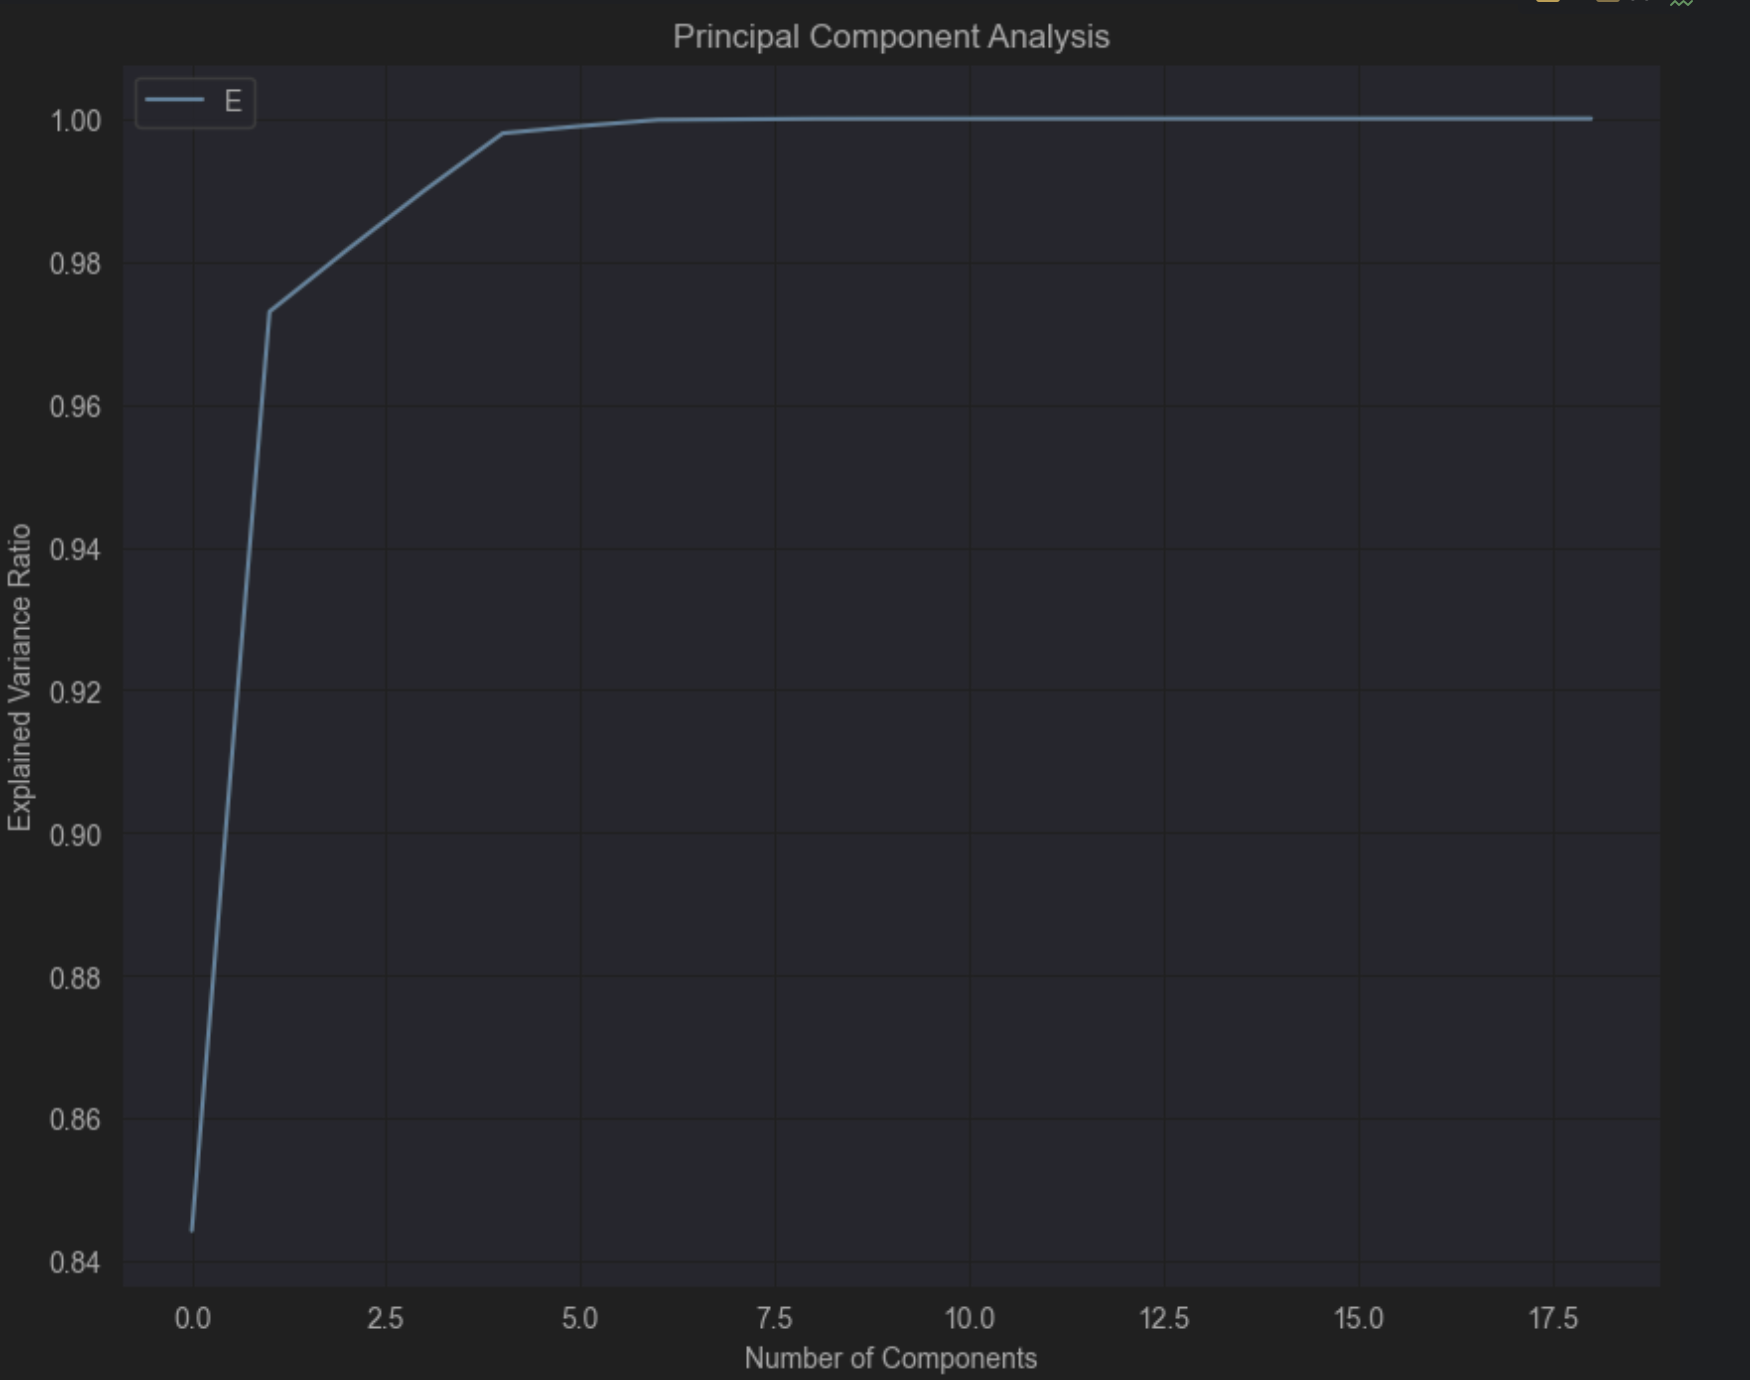
\includegraphics[width=0.8\textwidth]{./images/PCA_analyze}
  \caption{PCA's hyper parameter with encoding}
  \label{fig:PCA_encode}
\end{figure}

\begin{figure}
  \centering
  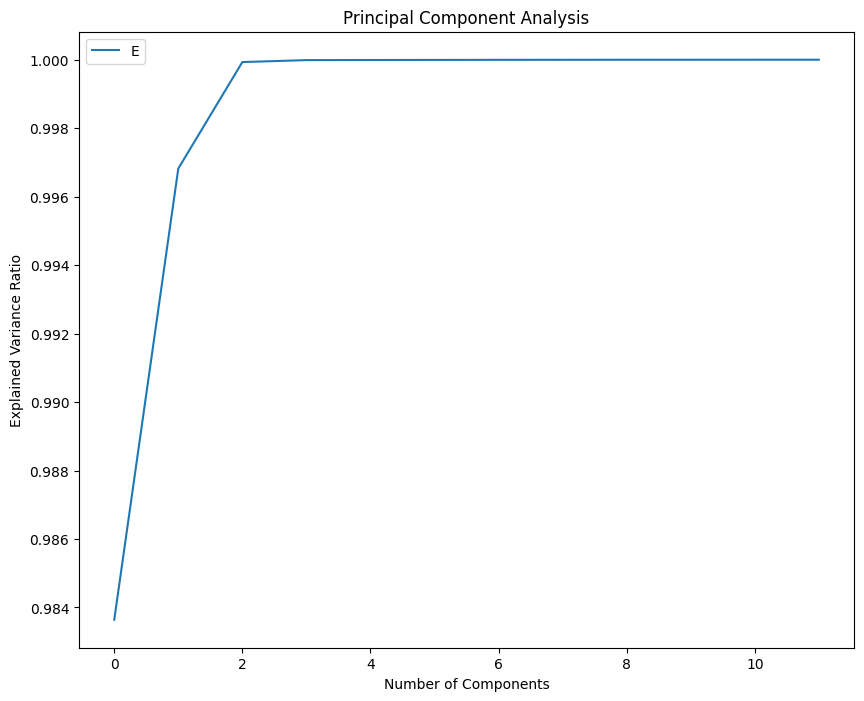
\includegraphics[width=0.8\textwidth]{./images/PCA_analyze_without_encoding.png}
  \caption{PCA's hyper parameter without encoding}
  \label{fig:PCA_without_encode}
\end{figure}

\subsubsection{Fine-tune winning feature}

The objective of our model is to predict the winners of various matches during a tournament. In the current state of our dataset, the model is configured to predict one of the following outcomes: a win for the home country, a loss for the home country (equivalent to a win for the away country), or a neutral result.\\

However, for our specific use case, we only want to predict wins or losses (not neutral outcomes) because, in a tournament format, matches cannot end in a neutral result.\\

Initially, we had 4628 neutral matches. We removed all neutral matches for friendly games, resulting in 2774 remaining neutral competitive matches. We then utilized data from "shootouts.csv" to determine the winners of these matches where possible, reducing the number to 2561 (mainly from qualifiers where shootouts were not applicable).\\

Considering the relatively small size of the neutral dataset and the absence of alternative solutions, we made the decision to exclude all neutral matches from our dataset.

\subsubsection{Imbalanced data}
Analysis reveal that classes are imbalanced: 
\begin{figure}[H]
  \centering
  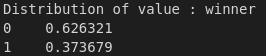
\includegraphics[width=0.5\textwidth]{./images/imbalanced.png}
  \caption{Imbalanced classes}
  \label{fig:imbalanced}
\end{figure}

This may introduce bias to the model which could struggle at predicting correctly the minority class.

To tackle this issue, a random oversampling is done on the minority class, duplicating random data from the minority class. This way, we get balanced classes. 

\begin{figure}[H]
  \centering
  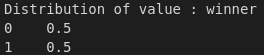
\includegraphics[width=0.5\textwidth]{./images/balanced.png}
  \caption{Balanced classes}
  \label{fig:balanced}
\end{figure}

However, as we will mention later, it may introduce overfitting as some data is redundant.

Nonetheless, there are more advanced techniques that are worth a try like SMOTE to deal with imbalanced data.
\subsection{Summary}

With the completion of all modifications and adjustments, our dataset is now prepared for further analysis. We have taken necessary steps to mitigate biases and address the curse of dimensionality. The dataset is now primed for training machine learning models.\\

Here's an overview of the features of the dataset preprocessed.

\begin{figure}[H]
  \centering
  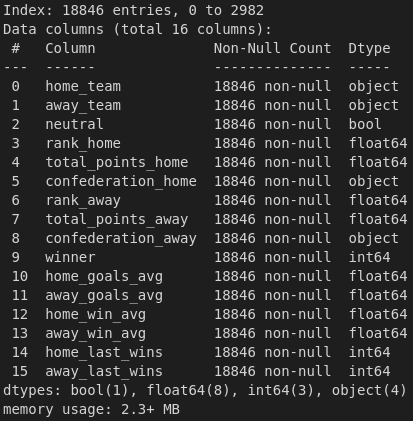
\includegraphics[width=0.7\textwidth]{./images/df_info.png}
  \caption{Preprocessed dataset features}
  \label{fig:dataset_features}
\end{figure}

\section{Models}

In this section, we will analyze the different models used to predict match results and the results obtained.\\
We train and evaluate three different kinds of models:
\begin{itemize}
    \item Random Forest
    \item Multi Layer Perceptron Classifier (MLPC)
    \item Logistic regression
\end{itemize}

All models are trained and evaluated using default hyperparameters \textbf{AND} optimized hyperparameters (Grid search).  
The data used (``rera.joblib'') has been preprocessed in the preprocessing notebook, as described before.
  
In the end, the goal is to choose the best model to predict match results during the competition.\\

Before training the model, features must be preprocessed:
\begin{itemize}
    \item Encode categorical features using one hot encoding method: models only deal with numbers, so we must convert non numbers features to numbers.
    \item Standardize numerical features: to avoid introducing bias related to different scales across columns. If a column has numbers much greater than other columns, the model may give more importance to this column, whereas it shouldn't.
\end{itemize}
If we want to feed the model with new data for prediction, this data must be preprocessed the same way as during training.

So, in order to anticipate and simplify the prediction phase, we used scikit-learn pipelines to include this preprocessing step during training and prediction.

Pipelines are objects that allow to define several steps and apply fit() and transform() methods on each of these steps sequentially. Each step must implement fit() and transform() methods.
In our case, the pipeline has 2 steps:
\begin{itemize}
    \item Preprocessing: contains standardization and one hot encoding steps.
    \item Classifier: contains the model.
\end{itemize}
This way, we can call the fit and predict methods on the Pipeline object, and both preprocessing and training or prediction are automatically executed, so we don't have to do the preprocessing manually each time we want to predict on new data.

The Pipeline \ref{fig:pipeline} object is then exported to joblib format, and we can use it in any program we want, without having to preprocess data again.\\

\begin{figure}[H]
  \centering
  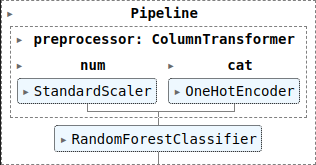
\includegraphics[width=0.5\textwidth]{./images/pipeline.png}
  \caption{Pipeline}
  \label{fig:pipeline}
\end{figure}

\textbf{Note}: for all the experiments, data is split the same way, i.e a third is dedicated to evaluation and two thirds for training. Models predict 2 classes : 0 (home team wins) and 1 (away team wins). A draw is predicted when predicted probabilities range between 0.45 and 0.55.
\subsection{Random Forest}

The first model trained is Random Forest.\\

Random Forest is an ensemble learning algorithm used for classification and regression in machine learning. It constructs multiple decision trees during training, where each tree is trained on a random subset of the data and considers a random subset of features at each decision point. The model outputs the mode of classes for classification or the mean prediction for regression based on individual tree outputs. This randomness and diversity help reduce overfitting, enhancing overall predictive performance. The final prediction is obtained by aggregating the predictions of all trees, resulting in a robust and versatile model known for high accuracy and generalization across diverse datasets.\\

\subsubsection{Default hyper-parameters}

The model is first trained using default hyper-parameters to get a baseline evaluation. Random state value is fixed to 42 to be able to reproduce the results.\\

Here's the confusion matrix obtained:

\begin{figure}[H]
  \centering
  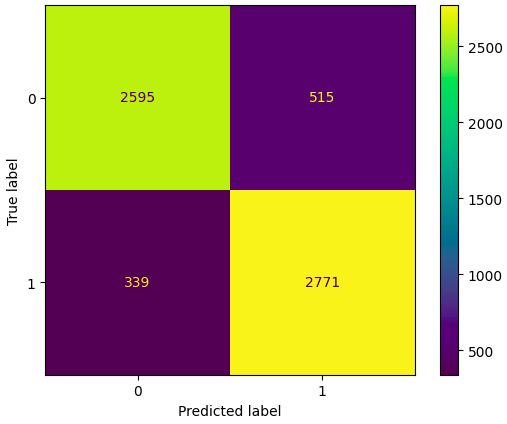
\includegraphics[width=0.7\textwidth]{./images/cm_rf_default.png}
  \caption{Confusion matrix rf default}
  \label{fig:cm_rf_default}
\end{figure}

The confusion matrix reveals that the model is a little bit better at predicting the class "1" corresponding to away team wins. This observation applies to all training configuration, and may be attributed to the oversampling done to get balanced classes (the minority class over-sampled is the class "1").\\

Evaluation metrics are reported in the classification report.

\begin{figure}[H]
  \centering
  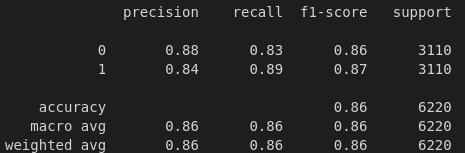
\includegraphics[width=0.7\textwidth]{./images/report_rf_default.png}
  \caption{Classification report rf default}
  \label{fig:report_rf_default}
\end{figure}

The accuracy score is pretty good: 0.86. The model has a good representation of the data and is able to extract interesting information from the features in order to predict the result of a match.\\

Nonetheless, learning curves \ref{fig:lc_rf_default} shows a not negligible gap between the validation and the training curves, indicating that the model is perhaps overfitting the data, and therefore may struggle to generalize to new data. (it's not sure because we don't see the curve going down)

\begin{figure}[H]
  \centering
  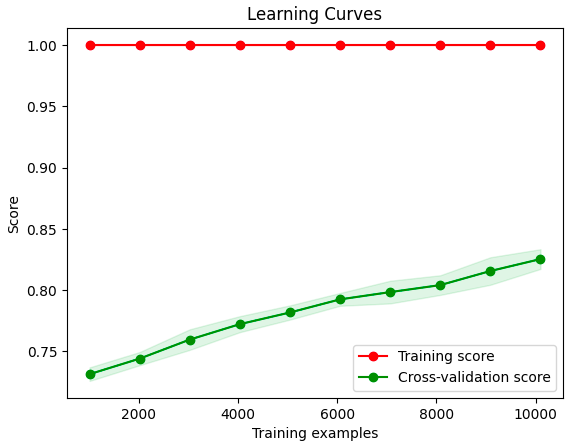
\includegraphics[width=0.7\textwidth]{./images/lc_rf_default.png}
  \caption{Learning curves rf default}
  \label{fig:lc_rf_default}
\end{figure}

It may be due to the random oversampling used to balance classes. By duplicating data, we must have influenced the model to overfit. 

It's also possible that it's due to the fact that the Random Forest is too complex to represent the data we're using.\\
  
As a consequence, it's likely that the model won't be able to generalize very well, even if the accuracy is high.\\ 
To address this issue, there are some avenues to explore:
\begin{itemize}
    \item Use another method for oversampling to balance the classes (like SMOTE algorithm).
    \item Further fine-tune the model hyperparameters.
    \item Use a simpler model like Logistic Regression.
\end{itemize}




\subsubsection{Fine-tuned hyper-parameters}


Model hyperparameters are the configuration settings used to structure and guide the learning process of a machine learning model. These hyperparameters are set before the training process and play an important role in model's performance improvement and overfitting/underfitting control.\\

Some examples of hyperparameters for Random Forest model are:
\begin{itemize}
    \item \textbf{n estimators}: refers to the number of trees in the forest. Generally, more trees increase the performance and make the predictions more stable, but they also make the computation slower.
    \item \textbf{max depth}: sets the maximum depth of each tree. Deeper trees can model more complex patterns but might lead to overfitting. Conversely, shallower trees might be too simplistic (underfitting).
    \item \textbf{max features}: determines the number of features to consider when looking for the best split during the construction of the trees.
\end{itemize}

There are other hyperparameters, but these ones seem to be a good starting point to optimize model's performance.\\

An exhaustive search to find the best configurations for these hyperparameters is not possible. Thus, it's required to define the hyperparameters search space:
\begin{itemize}
    \item \textbf{n estimators}: [50, 100, 500].
    \item \textbf{max depth}: [10, 50, 100].
    \item \textbf{max features}: [None, 'sqrt', 'log2'].
\end{itemize}

Using Grid Search CV from scikit-learn library, we can find the best hyperparameters combination in the defined search space.

For each combination of parameters in the search space, Grid Search CV performs K-fold cross-validation. This means the data is split into K subsets (folds); the model is trained on K-1 of these folds and validated on the remaining one. This process is repeated K times, with each fold being used once as the validation set. Cross-validation helps in assessing the model's performance more robustly, reducing the risk of overfitting on the training set.

After training on each combination, Grid Search CV evaluates the model's performance using a scoring metric, like accuracy.

Once all combinations have been evaluated, Grid Search CV selects the combination of parameters that yielded the best performance according to the chosen metric.

Finally, the model is retrained on the entire dataset using the best-found parameters.\\

Best hyperparameters values found:
\begin{figure}[H]
  \centering
  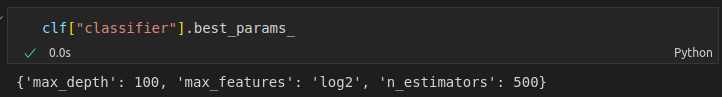
\includegraphics[width=0.9\textwidth]{./images/best_params.png}
  \caption{Best hyperparameters rf}
  \label{fig:best_params_rf}
\end{figure}

Unfortunately, the hyperparameters fine-tuning did not improve model's accuracy \ref{fig:report_rf_gridsearch}, nor did it help reduce the gap between training and validation curves \ref{fig:lc_rf_gridsearch}. 

Further experiments with different search spaces should be done to improve the results.

\begin{figure}[H]
  \centering
  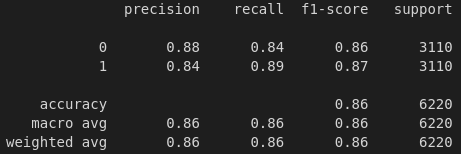
\includegraphics[width=0.7\textwidth]{./images/report_rf_gridsearch.png}
  \caption{Classification report rf gridsearch}
  \label{fig:report_rf_gridsearch}
\end{figure}

\begin{figure}[H]
  \centering
  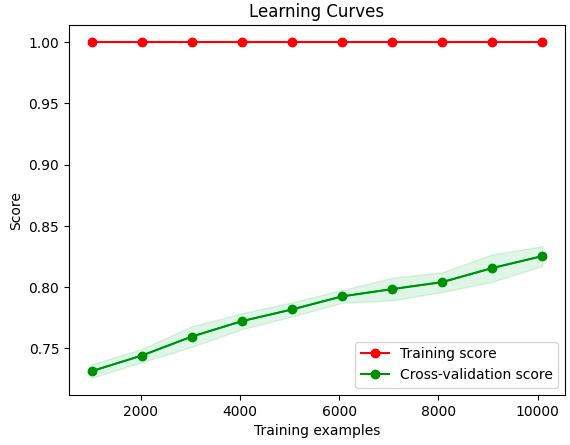
\includegraphics[width=0.7\textwidth]{./images/lc_rf_gridsearch.png}
  \caption{Learning curves rf gridsearch}
  \label{fig:lc_rf_gridsearch}
\end{figure}



\subsection{Multi-Layer Perceptron Classifier (MLPC)}


The Multi-Layer Perceptron Classifier (in scikit-learn) is a type of neural network model used for classification tasks. It belongs to the family of feedforward artificial neural networks and is used to solve problems that require supervised learning.\\

MLPC consists of at least three layers of nodes: an input layer, one or more hidden layers, and an output layer. Each node in the hidden layers is a neuron that uses a non-linear activation function, typically ReLU (Rectified Linear Unit).

Weights are adjusted trying to minimize the \textbf{cross entropy} (log loss function):
\begin{equation} \label{cross_entropy}
H(y, \hat{y}) = -\sum_{i} y_i \log(\hat{y}_i)
\end{equation}

This loss is a representation of the difference between predicted values and true values. By minimising this function, we improve the model's accuracy.\\

By default, the MLPC of scikit-learn uses the Adam (Adaptive Moment Estimation) optimizer to update weights minimising the loss function. This optimizer is well-known for its efficiency, as it allows to adjust the learning rate for each parameter of the model, making it adaptive and faster than other algorithms to converge to the minima of the loss function.


\subsubsection{Default hyperparameters}

Like Random Forest, the MLPC model is first trained using default hyper-parameters to get a baseline evaluation. Random state value is fixed to 42 to be able to reproduce the results.\\

\begin{figure}[H]
  \centering
  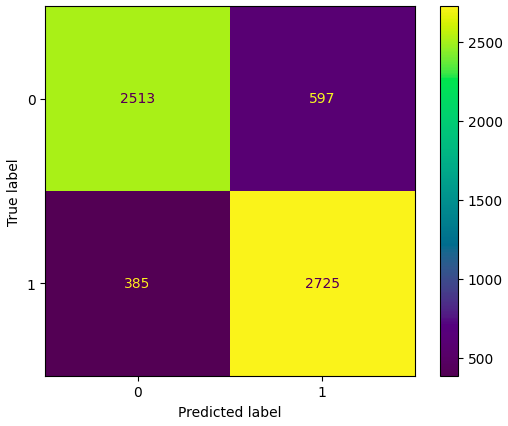
\includegraphics[width=0.7\textwidth]{./images/cm_mlpc_default.png}
  \caption{Confusion matrix mlpc default}
  \label{fig:cm_mlpc_default}
\end{figure}

Same observations as for Random Forest are made: the model is better at predicting the class "1" (when the away team wins) than "0" (when the home team wins).\\

Classification metrics results are reported in the classification report:

\begin{figure}[H]
  \centering
  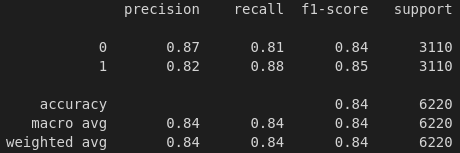
\includegraphics[width=0.7\textwidth]{./images/report_mlpc_default.png}
  \caption{Classification report mlpc default}
  \label{fig:report_mlpc_default}
\end{figure}

Results are a little bit worse than Random Forest (0.84 < 0.86), but still good.

However, like for Random Forest, learning curves suggest that the model may be overfitting:

\begin{figure}[H]
  \centering
  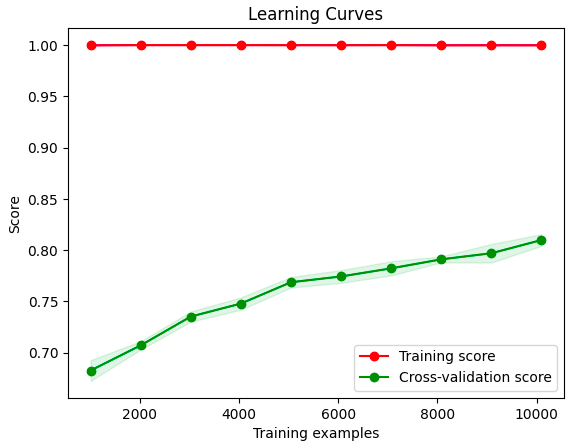
\includegraphics[width=0.7\textwidth]{./images/lc_mlpc_default.png}
  \caption{Learning curves mlpc default}
  \label{fig:lc_mlpc_default}
\end{figure}

Let's try to fine-tune the hyperparameters to improve the accuracy and reduce the gap between learning curves.

\subsubsection{Fine-tuned hyperparameters}

Like for Random Forest model, there are a lot of hyperparameters. For convenience and gain of time, we chose the following two hyperparameters to optimize:

\begin{itemize}
    \item \textbf{hidden layer sizes}: determines the size and number of hidden layers in the neural network. Overfitting often occurs when a model is too complex relative to the amount and complexity of the training data. By fine-tuning hidden layer sizes, we can control the model's complexity.
    \item \textbf{alpha}: L2 regularization term (also known as Ridge regularization) helps to avoid overfitting by penalizing large weights. Regularization adds a penalty to the loss function for complex models, encouraging simpler models that generalize better. A higher value of alpha increases the regularization effect, which means the optimizer prefers simpler models with smaller weights. This can prevent the model from fitting the training data too closely.
\end{itemize}


As said before, an exhaustive search is not possible and the time of computation required to run the grid search increases a lot when the search space is greater. We have to restrict to a relatively small search space (although we used njobs parameter to parallelize computations):
\begin{itemize}
    \item \textbf{hidden layer sizes}: [(50,), (100,), (50, 50)]
    \item \textbf{alpha}: [0.0001, 0.001, 0.01]
\end{itemize}

Best hyperparameters values found:

\begin{figure}[H]
  \centering
  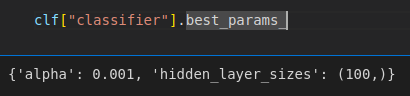
\includegraphics[width=0.7\textwidth]{./images/best_params_mlpc.png}
  \caption{Best hyperparameters values mlpc}
  \label{fig:best_params_mlpc}
\end{figure}

Like for Random Forest, the hyperparameters fine-tuning did not improve model’s accuracy \ref{fig:report_mlpc_gridsearch}, nor did it help reduce the overfitting \ref{fig:lc_mlpc_gridsearch}.

\begin{figure}[H]
  \centering
  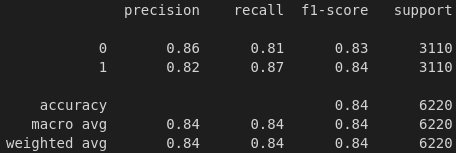
\includegraphics[width=0.7\textwidth]{./images/report_mlpc_gridsearch.png}
  \caption{Classification report mlpc gridsearch}
  \label{fig:report_mlpc_gridsearch}
\end{figure}

\begin{figure}[H]
  \centering
  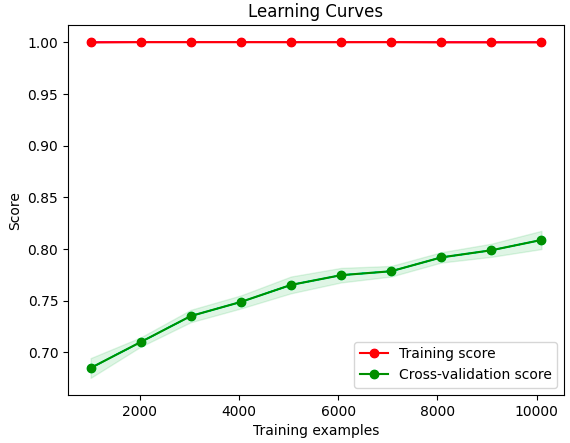
\includegraphics[width=0.7\textwidth]{./images/lc_mlpc_gridsearch.png}
  \caption{Learning curves mlpc gridsearch}
  \label{fig:lc_mlpc_gridsearch}
\end{figure}

\subsection{Logistic regression}

Logistic regression is a statistical method used for binary classification tasks. It's a type of regression analysis that's suitable for predicting the probability of a binary outcome (typically with two possible outcomes, like 'win' or 'loose', 'success' or 'failure', etc.).

It models the probability that a given input belongs to a particular category. It does this by using a logistic function to map predicted values to probabilities. This function outputs a value between 0 and 1, which can be interpreted as the probability of the instance belonging to a particular class.\\

Being a simpler model than Random Forest and MLPC, one can assume that it will not overfit the data, but at the risk of underfitting it.\\

Let's find out.\\

Here's the confusion matrix:
\begin{figure}[H]
  \centering
  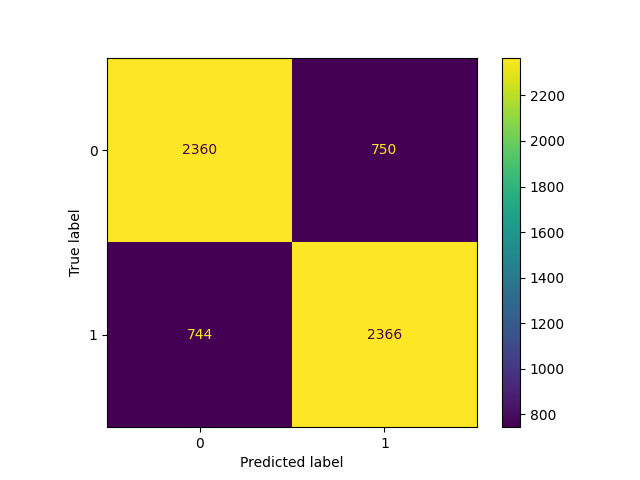
\includegraphics[width=0.7\textwidth]{./images/confusion_matrix_logistic.png}
  \caption{Confusion matrix logistic regression}
  \label{fig:cm_logistic}
\end{figure}

And the classification report:
\begin{figure}[H]
  \centering
  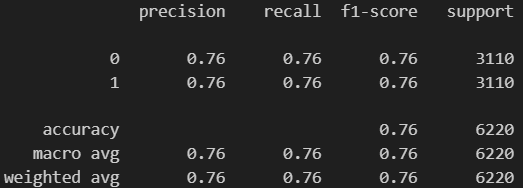
\includegraphics[width=0.7\textwidth]{./images/report_logistic.png}
  \caption{Classification report logistic regression}
  \label{fig:report_logistic}
\end{figure}

We observe that scores are lower than Random Forest and MLPC.\\

Let's have a look at the learning curves to check if the model is potentially overfitting or underfitting.
\begin{figure}[H]
  \centering
  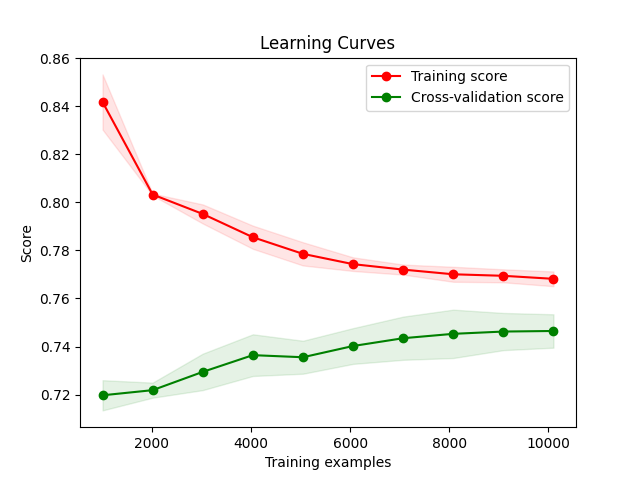
\includegraphics[width=0.7\textwidth]{./images/learning_curves_logistic.png}
  \caption{Learning curves logistic regression}
  \label{fig:lc_logistic}
\end{figure}

The gap between the curves is smaller, we're no more suspecting an overfitting, but the scores are also lower. Given the previous learning curves, we know that the training score can be really high, thus one can suspect an underfitting here, suggesting that the model is not good enough to correctly represent the data.\\






\subsection{Summary}

Although accuracy scores are pretty good, Random Forest and MLPC models have a non negligible gap between the training and the validation curves, which suggests a potential overfitting.

As a consequence, the model may not be able to generalize well.\\

As for the Logistic regression model, learning curves are close to each other, but scores are lower, suggesting a potential underfitting.\\

   
Hyperparameters fine-tuning did not help reduce the gap between learning curves, nor did it improve the accuracy. Further experiments with different search spaces should be done to improve the results.\\
  
As we're not sure about overfitting, we choose the model with the highest accuracy: Random Forest with optimized hyperparameters.\\

\textbf{Note}: MLPC model size is much smaller than Random Forest (1MB < < 49MB). But since memory is not really a constraint in our project, we still choose Random Forest.

\section{Python-Based User Interface for Predictive Models}

To better expose and allow users to test our models, we have implemented a Python-based user interface using Flask. The interface, hosted locally as a website, leverages the Flask library for seamless interaction.

\subsection{User Interface Structure}

The user interface comprises three distinct HTML pages: "Welcome," "Predict Match," and "Predict Tournament." Each page serves a unique purpose to enhance user experience.

\begin{itemize}
    \item \textbf{Welcome Page:} This initial page greets the user and provides the option to choose between the two prediction modes.
    \item \textbf{Predict Match Page:} Users can utilize this page to forecast match results.
    \item \textbf{Predict Tournament Page:} Designed in the FIFA World Cup format, this page allows users to set up a tournament and predict the eventual winner.
\end{itemize}

\subsection{Key Features}

The user interface incorporates several key features to improve usability and provide valuable insights:

\begin{itemize}
    \item \textbf{Auto-completion for Country Names:} To prevent typos and save time, the interface includes auto-completion functionality for country names.
    \item \textbf{Probability Display:} The interface dynamically displays the probability of a winner, conveying the likelihood of a team's success.
\end{itemize}

\subsection{Application Structure}

The entire application, along with all necessary files, is organized in the \textbf{app} directory. This directory contains the following subdirectories:

\begin{itemize}
    \item \textbf{assets:} Contains the models used in the user interface.
    \item \textbf{data:} Contains the data used in the file, specifically for the tournament.
    \item \textbf{static:} Contains the CSS file.
    \item \textbf{templates:} Contains the UI templates, encompassing the welcome page, match predictor page, and tournament predictor template.
    \item \textbf{app.py:} The main function driving the user interface.
    \item \textbf{predict\_match\_result.py:} Module containing functions to predict match results.
    \item \textbf{predict\_championship.py:} Module with functions to predict tournament winners.
\end{itemize}


\begin{figure}[H]
  \centering
  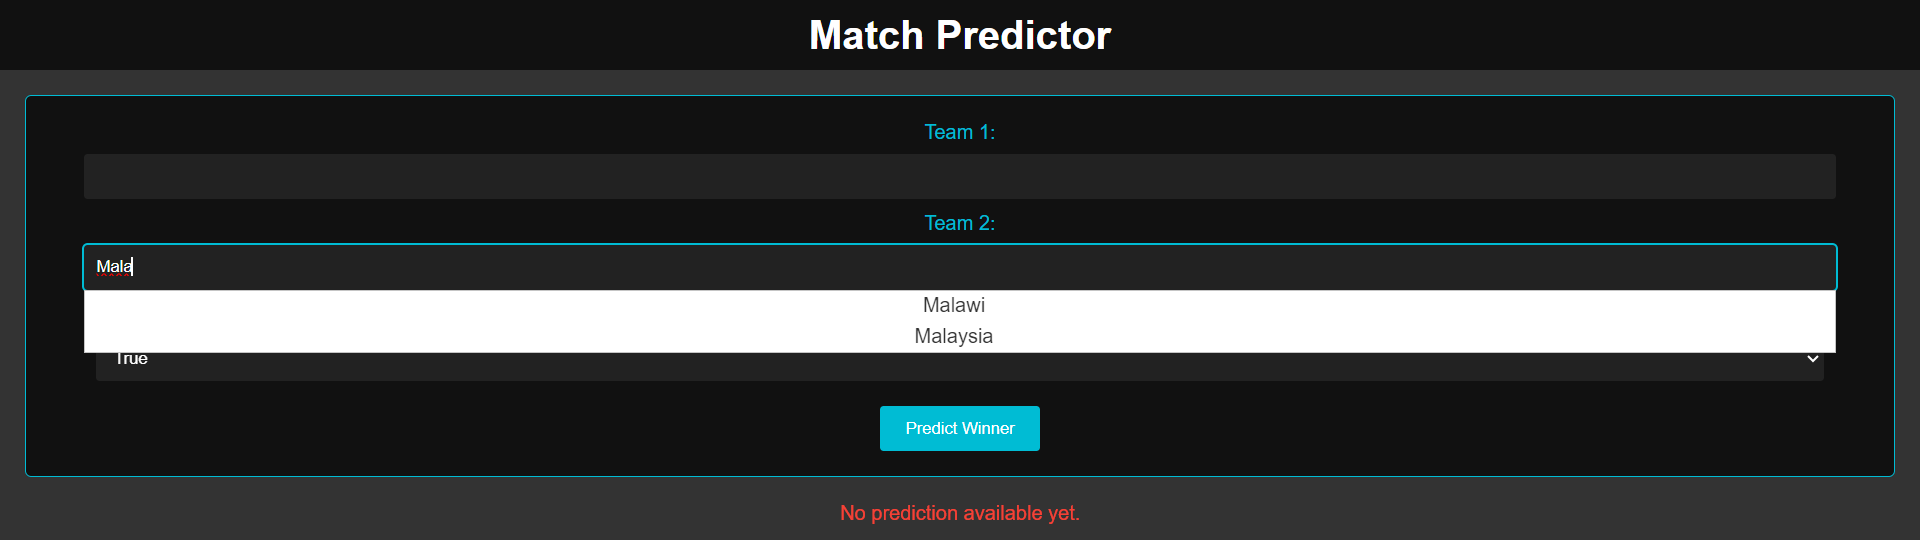
\includegraphics[width=1\textwidth]{./images/match_predictor.png}
  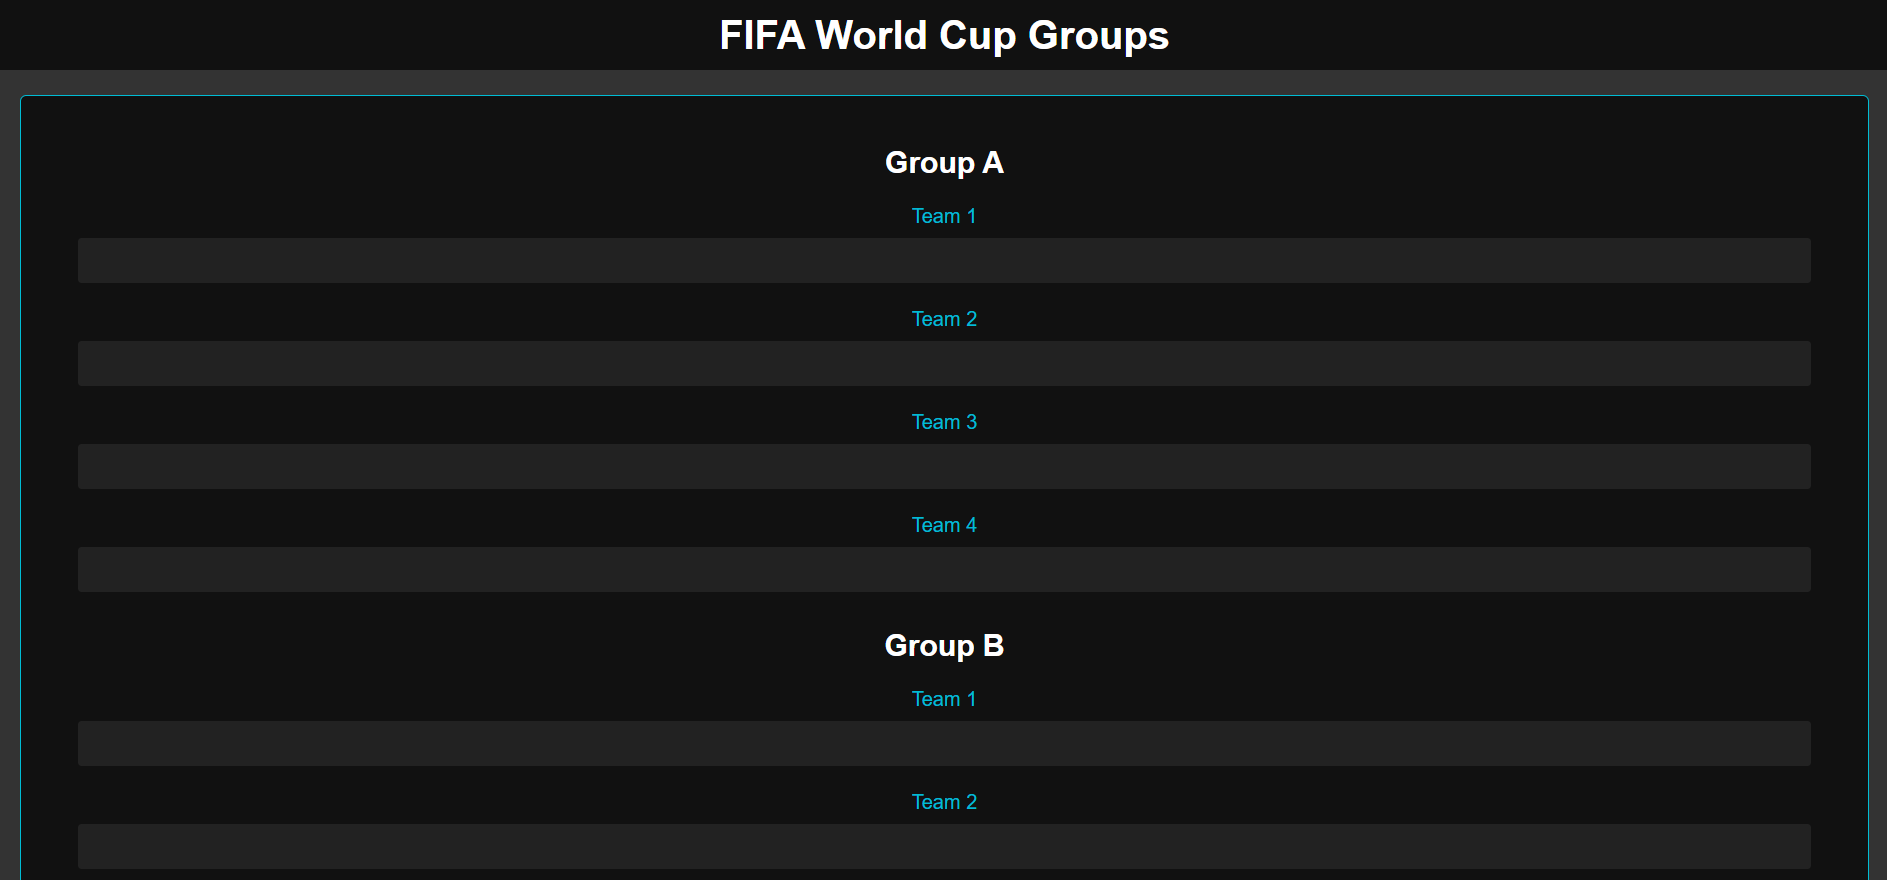
\includegraphics[width=1\textwidth]{./images/tournament_predict.png}
  \caption{Snaphshots of the UI}
  \label{fig:ui_match_predictor}
\end{figure}


\section{Conclusion}

The main purpose of this project is to be able to predict the result of football matches and the winner team of a championship.

To that end, scripts and a user interface allowing users to predict matches and championship results are provided.\\

We first preprocess the data in order to have relevant features compatible with the model input by:
\begin{itemize}
    \item Selecting a cutting year and standardizing country names to fit with current Fifa countries.
    \item Removing unrelevant features.
    \item Adding new relevant features.
    \item Standardizing numerical features and encoding the categorical ones to fit with the model constraints.
\end{itemize}

Then, we train several models with different configurations, evaluate them and choose the best model regarding the accuracy metric. Globally, accuracies are pretty good, but there's a large gap between the training and the validation curves for the Random Forest and the MLPC models, and a potential underfitting for the Logistic regression model. The performed analysis leads us to choose the Random Forest model.\\

Finally, we provide python scripts to predict the match result between 2 teams and the winner of a championship. We also provide a user interface to test these functionalities in a more user friendly way.\\


Given that it addresses nearly every aspect of machine learning, from data preprocessing to model deployment, working on this project was quite exciting. \\

The data preprocessing part seems to be the most challenging one since the model relies on the features coming from this data preprocessing, and it's not always easy to find the best way to clean and select relevant data to maximise the model performance. \\

Some improvements can be made to this project:
\begin{itemize}
    \item Try to preprocess data using different cutting years and compare the model performances.
    \item Find other relevant features to fit to the model.
    \item Compare more models with deeper hyperparameters optimization.
    \item Improve the user interface ergonomics.
\end{itemize}





\end{document}